\section{Introduction}

Many cognitive psychology researches have shown that given a visual scene, human attention is directed to particular parts by visual selective mechanism and these parts are called salient regions \cite{mangun1995neural}. In computer vision, salient region detection simulates the functionality of selective attention and localizes and tags the attention-grabbing regions or pixels in a digital image. Borji et al. \cite{borji2015salient} provided a more precise definition; they think that a salient region detection model should first detect the salient attention-grabbing objects in a context and then segment the whole objects. Usually, a generated saliency map is the output of the model and the intensity of each pixel in map means its probability of belonging to salient regions. According to this definition, we can know that this issue is essentially a figure/ground segmentation problem, and the goal is to only segment the salient foreground object from the background. However, it is slightly different from the traditional image segmentation problem that aims to partition an image into perceptually coherent regions.
Saliency detection for image is an important preprocessing step in many areas such as computer vision, graphics, and robotics to reduce computational cost by focusing on salient regions and neglecting the nonsalient. The value of salient region detection models lies on their wide applications, for instance, object detection and recognition \cite{ren2014region}, image and video compression \cite{guo2010novel}, thumb-nailing \cite{huang2011arcimboldo}, image quality assessment \cite{ li2013color}, image segmentation \cite{qin2014integration}, content based image retrieval \cite{feng2010attention}, and so on.



\noindent
Viewed from the information processing perspective, the existing models of visual saliency detection can be categorized as two main kinds: bottom-up and top-down. Bottom-up methods, also known as stimuli-driven or task-independent models, mainly detect saliency based on low-level feature attributes (color, orientation, motion, etc.) without any prior knowledge. Top-down approaches are often task-driven or scene-dependent models learning through training process, which requires some specific prior knowledge or high-level information. The human brains can perform this detection very quickly, and doing so on a computer remains a great challenge for researchers and scientists.


\section{Background}
The history of modern photography started many years back earlier in the 19th century. America’s history was filmed during the civil war with that in black and white. Many progressions have been made since then like digitization in photography.Kodak started to work on film-less technology in mid 70. At 1990 the commercial selling of digital cameras hits the road. The main benefit of storing the photographs in digital format is that these can be easily changed, reproduced and manipulated using different mathematic and computational algorithms. The Field of image processing is continually evolving. During the past five years, there has been a significant increase in the level of interest in image morphology, neural networks, full-color image processing, image data compression, image recognition, and knowledge-based image analysis systems. Image processing methods stems from two principal application areas: improvement of pictorial information for human interpretation, and processing of scene data for autonomous machine perception. Image is better than any other information form for our human being to perceive. 
\begin{figure}[here]%
    \centering
    \subfloat[Original image]{{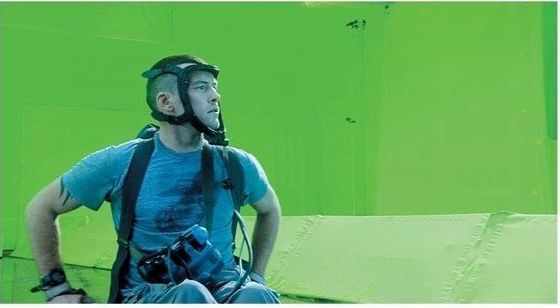
\includegraphics[width=0.45\textwidth,height=0.3\textwidth]{pictures/avatar1.jpg} }}%
    \qquad
    \subfloat[after processing]{{
\includegraphics[width=0.45\textwidth,height=0.3\textwidth]{pictures/avatar2.jpg} }}%
    \caption{Applications of Background and Foreground Segregation in Movies \protect\footnotemark}%
    \label{superpixel}%
\end{figure}
 \footnotetext{https://i.pinimg.com/564x/da/5c/b4/da5cb4e048759581f48f145ded236ca6.jpg}
Vision allows humans to perceive and understand the world surrounding us. Image understanding, image analysis, and computer vision aim to duplicate the effect of human vision by electronically (= digitally, in the present context) perceiving and understanding image(s)In digital image processing system, first step in the process is Image Acquisition it require acquiring an image, After a digital image has been obtained, the next step deals with Preprocessing its function is to improve the image in ways that increase the chance for success of the other processes, the next step deals with Segmentation it partitions an input image into its constituent parts or objects, Representation & Description deals with make data in the form that suitable for computer processing, and after that Recognition is that assigns a label to an object, and last Interpretation involves meaning to an assemble of recognized objects.

This thesis work focuses on one important problem in computational photography namely visually salient region detection. It is a primary job that needs to be done smoothly before doing most of the other digital image processing related job. With the rapid increase in technology involved with images, need for detection of visually salient region efficiently is also increasing.For example We know that movies, dramas and other entertaining videos happens to contain amazing stuffs and stunts like acting on the space or in big ship in an ocean. Even though they seem impossible to film in there, they seem so realistic. How do they do that? Well, there’s a little trick in there. It’s not that they’re acted in that scene. Rather, that background of that scene was added by segregating background from the salient region and other post processing. 


 



\section{Problem statement}
There are many existing systems for visually salient region detection. Most researches related to visual attention are driven by local or global contrast on low-level stimulus, such as intensity, color, and orientation.
A common technique is to compare each regions color difference with other regions of the image and the region having more color difference than other regions are more likely to be the attention region.
some research also focuses on the spacial distribution of regions. These researches assume that the salient region are more likely to be on the center of the image than being the regions that touches the boundary.
As visually salient region detection which consists of foreground extraction and background subtraction is a far from perfect art, there are several problems one needs to take into account when developing visually salient region detection algorithms. The following common problems are:

\subsection{Camouflage}
When a foreground object has the same texture or color characteristics as the background, allowing the object to blend into the background.In that case if we compare a salient regions color with background region it doesn't give significant color difference so that we can identify that salient region  

\begin{figure}[here]
  \centering
  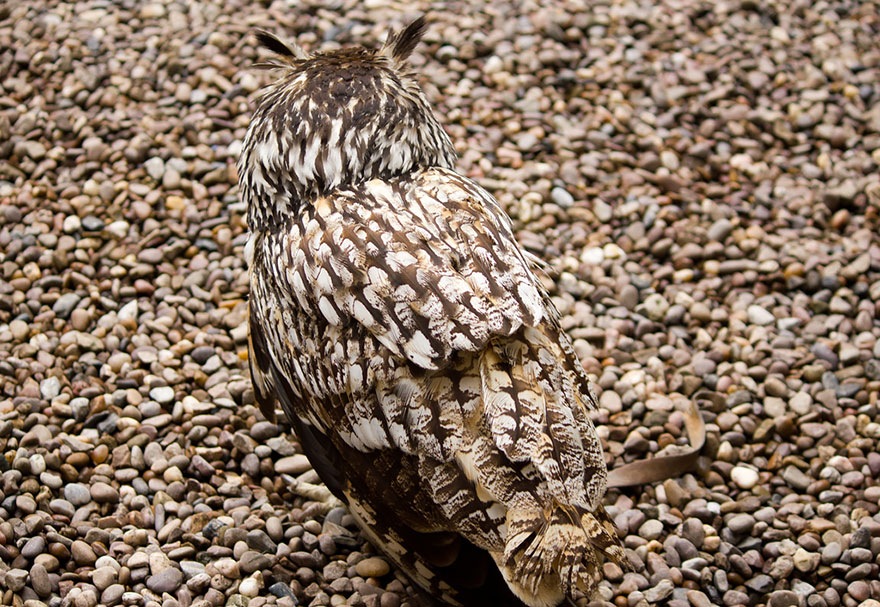
\includegraphics[width=0.55\textwidth,height=0.5\textwidth]{pictures/owl.jpg}
  \caption{Camouflage problem \protect\footnotemark}
  
  \label{orangeleaf}

\end{figure}
 \footnotetext{http://www.wikilinks.fr/wp-content/uploads/2013/06/camouflage-mimetisme-animal-camouflage-5.jpg}
 
\subsection{Partial matching color}
If part of a foreground object has same color as background,then differentiating full part of foreground with background becomes tough.


 
 
\begin{figure}[here]
  \centering
  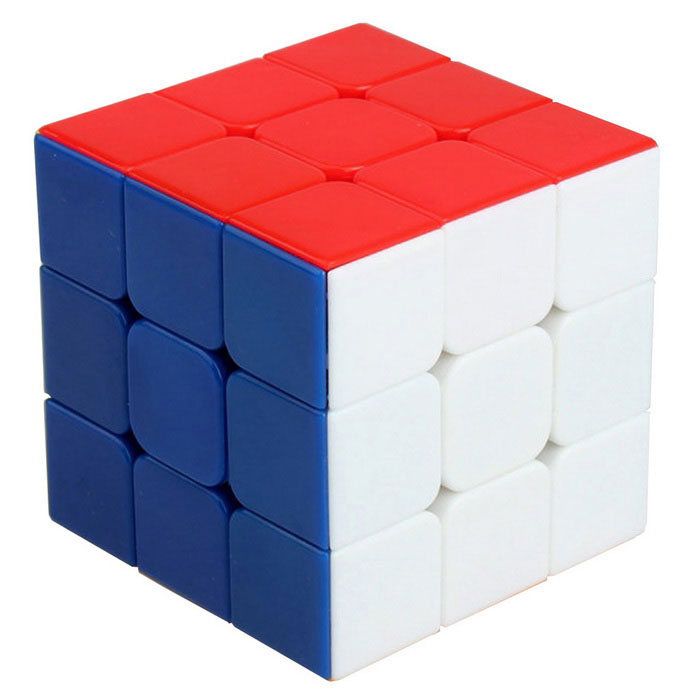
\includegraphics[width=0.55\textwidth,height=0.5\textwidth]{pictures/rubik.jpg}
  
  \caption{partial matching color problem \protect\footnotemark}
  
  \label{partial matching color}

\end{figure} 


 \footnotetext{http://img.dxcdn.com/productimages/sku_431118_1.jpg}

\subsection{Framed boundary}
If the boundary regions have frame with same color as foreground object then it becomes a difficult task to extract the salient region from it.

\begin{figure}[here]
  \centering
  
\includegraphics[width=0.35\textwidth,height=0.5\textwidth]{pictures/fork.jpg}
  
  \caption{partial matching color problem \protect\footnotemark}
  
  \label{partial matching color}

\end{figure} 

 \footnotetext{https://www.starvingartistframing.com/s/cc_images/cache_2850894204.jpg?t=1285712335}

\section{Motivation}
Saliency detection is an important preprocessing step in many application fields such as computer vision, robotics, and graphics. It reduces huge amount of computational cost by focusing on significant positions and neglecting the nonsignificant in the scene. So Most fields success depends on successful extraction of salient region from images. As human if we want to interact with the world then our eye becomes one of the most important part of our body. So in automated systems where we want to make the computer do humans job, we have to build something that acts as eye for the computer. using that eye computer will be able to see and understand things and make further decisions. As we know our brain tends to catch only the important region and ignore other regions surrounding it. It serves many purpose like understanding the situation faster and eliminating unnecessary computations and keep focus on the salient region. If we can simulate this wonderful characteristic of our eye and brain into a computer then it's going to be very helpful in real life applications of computers. For example for automated cars, drones and other unmanned vehicles faster scene analysis is a key requirement. visually salient region detection serves this purpose to simulate this wonderful characteristic of human eye for computer.

\section{Objectives}
The basic objective of this thesis is to make a robust system that can automatically detect and extract visually salient region from images
There is not any absolute system that can do this in complete manner. The main objectives of this thesis work are:
\begin{itemize}
  \item A detailed study on detection and extraction of visually salient region from images.
  \item To give a new idea on salient region detection.
  \item Implement and analyze performance on the proposed scheme based on accuracy, precision and recall.
\end{itemize}


 
\section{Organization of the thesis}
The rest of the thesis is organized as follows:
\begin{itemize}
  \item Chapter 2: This chapter discusses the literature surveys that have been done during this thesis. It also provides detailed survey of the literature related to visual saliency. Discussion about the existing and some new methods for salient region detection are done. This chapter presents the methodology and implementation of some existing and experimental results subsequently.
  \item Chapter 3: A new scheme for foreground extraction is proposed in here which uses color and spatial information of each region. A detailed study on visual saliency with our approach is discussed in here
  
  \item Chapter 4:The experimental outcomes of our proposed method along with necessary figures are discussed in details in this Chapter.
  \item Chapter 5:Recommendation for the future researchers of this work on the proposed model and the conclusive words about the model are outlined in this chapter.
  
\end{itemize}


 

  
\section{Conclusion}
In this chapter, we presented some background of digital image processing and a brief introduction of techniques for visually salient region detection.this chapter also discusses the basic objective of this thesis and the problems that needed to be taken into account when developing this algorithm